% Chapitre 3 : Calcul littéral (I) - Expressions et développement
% Conforme à la réforme du collège 2025
% Note: Ce document nécessite les packages tikz, amsmath, amssymb et les environnements personnalisés définis dans le préambule

\chapter{Calcul littéral (I) : Expressions et simple distributivité}

\section{Introduction}

Le calcul littéral est le langage universel des mathématiques. Il permet d'exprimer des relations générales, de modéliser des situations et de résoudre des problèmes complexes.

\subsection*{Un peu d'histoire}
\begin{itemize}
	\item \textbf{Al-Khwarizmi (IXe siècle)} : Père de l'algèbre, introduit la résolution systématique d'équations.
	\item \textbf{François Viète (XVIe siècle)} : Premier à utiliser des lettres pour représenter des nombres inconnus et connus.
	\item \textbf{René Descartes (XVIIe siècle)} : Normalise l'usage de $x$, $y$, $z$ pour les inconnues et $a$, $b$, $c$ pour les paramètres.
\end{itemize}

\textbf{Problématique du chapitre :} Comment traduire une situation par une expression mathématique ? Comment simplifier et transformer des expressions pour faciliter les calculs ?

\section{Activité — Du langage courant au langage mathématique}

\begin{objectifsbox}
	\begin{itemize}
		\item[\textbullet] Traduire une situation concrète en expression littérale
		\item[\textbullet] Comprendre l'utilité des lettres en mathématiques
		\item[\textbullet] Découvrir les règles de simplification
	\end{itemize}
\end{objectifsbox}

\subsection*{Situation 1 : Le périmètre d'un terrain}

\begin{activitybox}[Les dimensions variables]
	Un terrain rectangulaire a une longueur de 20 mètres de plus que sa largeur.
	
	\begin{enumerate}
		\item Si la largeur mesure 30 m, quelle est la longueur ? \trous{3cm}
		\item Si la largeur mesure 45 m, quelle est la longueur ? \trous{3cm}
		\item Si on note $\ell$ la largeur, comment exprimer la longueur ? \trous{5cm}
		\item Exprimer le périmètre du terrain en fonction de $\ell$ : \trous{8cm}
		\item Simplifier cette expression : \trous{8cm}
	\end{enumerate}
\end{activitybox}

\subsection*{Situation 2 : Tarifs et réductions}

\begin{activitybox}[Modélisation d'une situation commerciale]
	Un magasin propose une réduction de 20\% sur tous les articles.
	
	\begin{enumerate}
		\item Si un article coûte 50€, quel est son prix après réduction ? \trous{3cm}
		\item Si un article coûte $p$ euros, exprimer :
		\begin{itemize}
			\item Le montant de la réduction : \trous{5cm}
			\item Le prix après réduction : \trous{5cm}
		\end{itemize}
		\item Simplifier l'expression du prix après réduction : \trous{5cm}
	\end{enumerate}
\end{activitybox}

\section{Vocabulaire et notations}

\begin{definitionbox}[Expression littérale]
	Une \textbf{expression littérale} est une expression mathématique comportant une ou plusieurs lettres qui représentent des nombres.
	
	\textbf{Exemples :} $3x + 5$, $2a - b$, $x^2 + 2x - 3$
	
	Les lettres utilisées sont appelées \textbf{variables} ou \textbf{inconnues}.
\end{definitionbox}

\begin{vocabulairebox}[Terminologie du calcul littéral]
	\begin{itemize}
		\item \textbf{Terme} : Partie d'une expression séparée par + ou -
		\begin{itemize}
			\item[\textbullet] Dans $3x + 5y - 2$, les termes sont : \solution{$3x$}, \solution{$5y$} et \solution{$-2$}
		\end{itemize}
		\item \textbf{Coefficient} : Nombre qui multiplie une variable
		\begin{itemize}
			\item[\textbullet] Dans $7x$, le coefficient est \solution{7}
			\item[\textbullet] Dans $-3y$, le coefficient est \solution{-3}
			\item[\textbullet] Dans $x$, le coefficient est \solution{1} (sous-entendu)
		\end{itemize}
		\item \textbf{Partie littérale} : La ou les lettres d'un terme
		\begin{itemize}
			\item[\textbullet] Dans $5xy$, la partie littérale est \solution{$xy$}
		\end{itemize}
		\item \textbf{Terme constant} : Terme sans variable
		\begin{itemize}
			\item[\textbullet] Dans $2x + 8$, le terme constant est \solution{8}
		\end{itemize}
	\end{itemize}
\end{vocabulairebox}

\begin{remarkbox}[Conventions d'écriture]
	\begin{itemize}
		\item[\textbullet] Le signe $\times$ est souvent omis : $3 \times x = 3x$
		\item[\textbullet] $1 \times x = x$ (on n'écrit pas le coefficient 1)
		\item[\textbullet] $-1 \times x = -x$ (on n'écrit pas le coefficient -1)
		\item[\textbullet] Entre deux lettres : $a \times b = ab$
		\item[\textbullet] Ordre alphabétique préféré : $xy$ plutôt que $yx$
	\end{itemize}
\end{remarkbox}

\section{Calculer la valeur d'une expression}

\begin{definitionbox}[Substitution]
	\textbf{Substituer}, c'est remplacer une lettre par une valeur numérique donnée.
	
	Pour calculer la valeur d'une expression littérale :
	\begin{enumerate}
		\item Remplacer chaque lettre par sa valeur
		\item Respecter les priorités opératoires
		\item Effectuer les calculs
	\end{enumerate}
\end{definitionbox}

\begin{methodebox}[Calculer une valeur numérique]
	\textbf{Étapes à suivre :}
	\begin{enumerate}
		\item Réécrire l'expression en remplaçant les lettres par leurs valeurs (entre parenthèses si nécessaire)
		\item Appliquer les priorités : Parenthèses → Puissances → Multiplications/Divisions → Additions/Soustractions
		\item Calculer progressivement
	\end{enumerate}
\end{methodebox}

\begin{examplebox}[Substitution simple]
	Calculer $A = 3x - 5$ pour $x = 4$
	
	\textbf{Solution :}
	\begin{align*}
		A &= 3x - 5\\
		A &= ..........\\
		A &= ...........\\
		A &= ...........
	\end{align*}
\end{examplebox}

\begin{examplebox}[Substitution avec plusieurs variables]
	Calculer $B = 2a + 3b - ab$ pour $a = 5$ et $b = -2$
	
	\textbf{Solution :}
	\begin{align*}
		B &= 2a + 3b - ab\\
		B &= .......................................\\
		B &= ............................\\
		B &= ............................\\
		B &= ............................
	\end{align*}
\end{examplebox}

\begin{attentionbox}[Piège des nombres négatifs]
	Attention lors de la substitution de nombres négatifs !
	
	Si $x = -3$ :
	\begin{itemize}
		\item $x^2 = (-3)^2 = 9$ (et non pas $-9$)
		\item $2x = 2 \times (-3) = -6$
		\item $-x = -(-3) = 3$
	\end{itemize}
	
	\textbf{Conseil :} Mettre les nombres négatifs entre parenthèses lors de la substitution.
\end{attentionbox}

\section{Simplifier et réduire une expression}

\subsection{Simplifier une écriture}

\begin{definitionbox}[Simplification]
	\textbf{Simplifier} une expression, c'est l'écrire de la manière la plus concise possible en respectant les conventions mathématiques.
\end{definitionbox}

\begin{examplebox}[Simplifications courantes]
	\begin{center}
		\begin{tabular}{|l|l|l|}
			\hline
			\textbf{Écriture non simplifiée} & \textbf{Écriture simplifiée} & \textbf{Règle appliquée} \\
			\hline
			$1 \times x$ & $x$ & Coefficient 1 omis \\
			\hline
			$x \times 3$ & $3x$ & Coefficient devant \\
			\hline
			$x \times y$ & $xy$ & Signe $\times$ omis \\
			\hline
			$x + (-5)$ & $x - 5$ & Simplification des signes \\
			\hline
			$0 \times x$ & $0$ & Multiplication par 0 \\
			\hline
			$x + 0$ & $x$ & Addition de 0 \\
			\hline
		\end{tabular}
	\end{center}
\end{examplebox}

\subsection{Réduire une expression}

\begin{definitionbox}[Réduction]
	\textbf{Réduire} une expression, c'est regrouper les termes qui ont la même partie littérale (termes semblables).
\end{definitionbox}

\begin{proprietebox}[Termes semblables]
	Deux termes sont semblables s'ils ont exactement la même partie littérale.
	
	\textbf{Exemples :}
	\begin{itemize}
		\item $3x$ et $5x$ sont semblables (partie littérale : $x$)
		\item $2xy$ et $-7xy$ \solution[5cm]{sont semblables (partie littérale : $xy$)}
		\item $4x$ et $4y$ \solution[6cm]{ne sont PAS semblables}
		\item $3x^2$ et $3x$ \solution[6cm]{ne sont PAS semblables}
	\end{itemize}
\end{proprietebox}

\begin{methodebox}[Réduire une expression]
	\textbf{Méthode systématique :}
	\begin{enumerate}
		\item Identifier les termes semblables (même partie littérale)
		\item Les regrouper mentalement ou les souligner de la même couleur
		\item Additionner ou soustraire leurs coefficients
		\item Écrire l'expression réduite
	\end{enumerate}
\end{methodebox}

\begin{examplebox}[Réduction guidée]
	Réduire $E = 5x + 3y - 2x + y - 4$
	
	\textbf{Solution détaillée :}
	\begin{itemize}
		\item Termes en $x$ : $5x$ et $-2x$ → $(5 - 2)x = 3x$
		\item Termes en $y$ : $3y$ et $y$ → $(3 + 1)y = 4y$
		\item Terme constant : $-4$
		\item \textbf{Résultat :} $E = 3x + 4y - 4$
	\end{itemize}
\end{examplebox}

\begin{examplebox}[Réduction complexe]
	Réduire $F = 2a^2 + 3a - 5 + a^2 - 7a + 2$
	
	\textbf{Solution :}
	\begin{itemize}
		\item Termes en $a^2$ : \solution{$2a^2$} et \solution{$a^2$} → \solution{$(2 + 1)a^2 = 3a^2$}
		\item Termes en $a$ : \solution{$3a$} et \solution{$-7a$} → \solution{$(3 - 7)a = -4a$}
		\item Termes constants : \solution{$-5$} et \solution{$2$} → \solution{$-5 + 2 = -3$}
		\item \textbf{Résultat :} $F = \solution{3a^2 - 4a - 3}$
	\end{itemize}
\end{examplebox}

\section{Développer avec la distributivité simple}

\begin{definitionbox}[Développer une expression]
	\textbf{Développer} une expression, c'est transformer un produit en une somme algébrique.

	On passe d'une forme factorisée (produit) à une forme développée (somme).

	\textbf{Exemple :} $2(x + 3)$ (produit) $\longrightarrow$ $2x + 6$ (somme)
\end{definitionbox}

\begin{examplebox}[Pourquoi développer ?]
	Calculer $3(x + 5)$ pour $x = 2$ :

	\textbf{Méthode 1 (sans développer) :}
	$$\solution{3(2 + 5)} = \solution{3 \times 7 = 21}$$

	\textbf{Méthode 2 (en développant) :}
	$$3(x + 5) = \solution{3x + 15}$$
	donc pour $x = 2$ : $3 \times 2 + 15 = 6 + 15 = 21$
	
	Développer permet de transformer l'expression et facilite certains calculs ultérieurs.
\end{examplebox}

\subsection{La propriété de distributivité}

\begin{proprietebox}[Distributivité de la multiplication]
	Pour tous nombres $k$, $a$ et $b$ :
	\begin{itemize}
		\item $k(a + b) = ka + kb$ \quad (distributivité sur l'addition)
		\item $k(a - b) = ka - kb$ \quad (distributivité sur la soustraction)
	\end{itemize}

	\textbf{Visualisation géométrique :}
	\begin{center}
		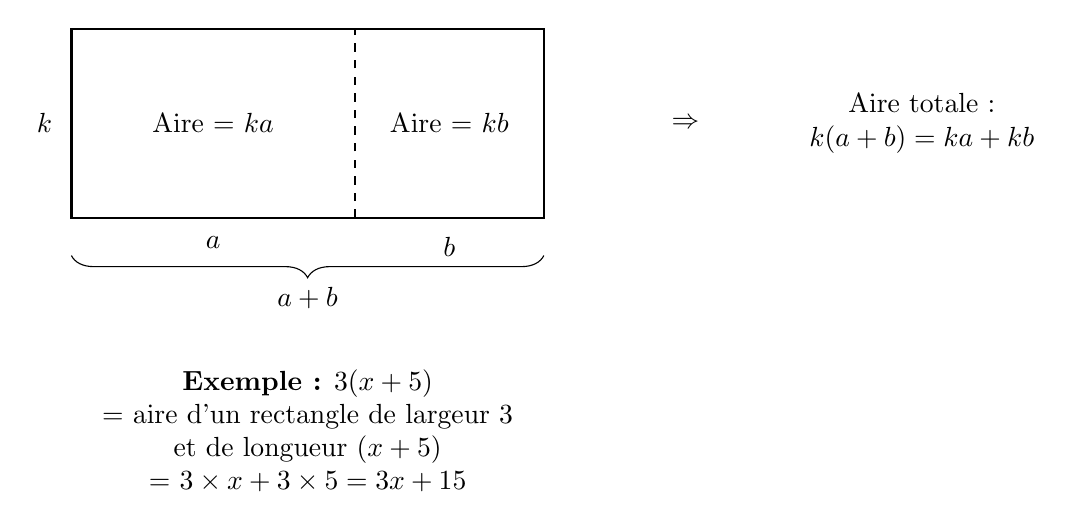
\begin{tikzpicture}[scale=1.2]
			% Rectangle principal
			\draw[thick] (0,0) rectangle (5,2);

			% Séparation verticale
			\draw[dashed, thick] (3,0) -- (3,2);

			% Labels des dimensions
			\node[below] at (1.5,-0.1) {$a$};
			\node[below] at (4,-0.1) {$b$};
			\node[left] at (-0.1,1) {$k$};

			% Accolades pour montrer a+b
			\draw[decorate, decoration={brace, amplitude=8pt, mirror}]
				(0,-0.4) -- (5,-0.4) node[midway, below, yshift=-8pt] {$a + b$};

			% Labels des aires
			\node at (1.5,1) {Aire = $ka$};
			\node at (4,1) {Aire = $kb$};

			% Flèche et égalité
			\node at (6.5,1) {$\Rightarrow$};
			\node[align=center] at (9,1) {Aire totale :\\ \solution{$k(a+b) = ka + kb$}};

			% Exemple numérique en dessous
			\node[below, align=center] at (2.5,-1.5) {
				\textbf{Exemple :} $3(x + 5)$\\
				= aire d'un rectangle de largeur 3\\
				et de longueur $(x + 5)$\\
				= $3 \times x + 3 \times 5 = 3x + 15$
			};
		\end{tikzpicture}
	\end{center}
\end{proprietebox}

\begin{remarkbox}[Sens de lecture]
	\begin{itemize}
		\item \textbf{Développer :} passer de $k(a + b)$ à $ka + kb$
		\item \textbf{Factoriser :} passer de $ka + kb$ à $k(a + b)$ (vu plus tard)
	\end{itemize}
\end{remarkbox}

\begin{methodebox}[Développer une expression]
	Pour développer $k(a + b)$ :
	\begin{enumerate}
		\item Multiplier $k$ par chaque terme dans la parenthèse
		\item Respecter la règle des signes
		\item Simplifier si possible
		\item Réduire l'expression obtenue
	\end{enumerate}
\end{methodebox}

\begin{examplebox}[Développement simple]
	Développer $A = 3(x + 5)$
	
	\textbf{Solution :}
	\begin{align*}
		A &= 3(x + 5)\\
		A &= \solution{3 \times x + 3 \times 5}\\
		A &= \solution{3x + 15}
	\end{align*}
\end{examplebox}

\begin{examplebox}[Développement avec soustraction]
	Développer $B = 4(2x - 3)$
	
	\textbf{Solution :}
	\begin{align*}
		B &= 4(2x - 3)\\
		B &= \solution{4 \times 2x - 4 \times 3}\\
		B &= \solution{8x - 12}
	\end{align*}
\end{examplebox}

\begin{examplebox}[Développement avec coefficient négatif]
	Développer $C = -2(3x + 4)$
	
	\textbf{Solution :}
	\begin{align*}
		C &= -2(3x + 4)\\
		C &= \solution{-2 \times 3x + (-2) \times 4}\\
		C &= \solution{-6x - 8}
	\end{align*}
\end{examplebox}

\begin{attentionbox}[Erreurs fréquentes]
	\begin{center}
		\begin{tabular}{|l|l|l|}
			\hline
			\textbf{Erreur} & \textbf{Faux} & \textbf{Correct} \\
			\hline
			Oubli d'un terme & $3(x + 2) = 3x$ & $3(x + 2) =$ \solution{$3x + 6$} \\
			\hline
			Erreur de signe & $-2(x - 3) = -2x - 6$ & $-2(x - 3) =$ \solution{$-2x + 6$} \\
			\hline
			Distribution partielle & $2(3x + 4y) = 6x + 4y$ & $2(3x + 4y) = \solution{6x + 8y}$ \\
			\hline
		\end{tabular}
	\end{center}
\end{attentionbox}

\subsection{Développement et réduction}

\begin{methodebox}[Développer puis réduire]
	Quand une expression contient plusieurs développements :
	\begin{enumerate}
		\item Développer chaque produit séparément
		\item Supprimer toutes les parenthèses
		\item Identifier les termes semblables
		\item Réduire l'expression
	\end{enumerate}
\end{methodebox}

\begin{examplebox}[Exemple complet]
	Développer et réduire $D = 3(x + 2) + 2(x - 4)$
	
	\textbf{Solution détaillée :}
	\begin{align*}
		D &= 3(x + 2) + 2(x - 4)\\
		&= 3x + 6 + 2x - 8 \quad \text{(développement)}\\
		&= 3x + 2x + 6 - 8 \quad \text{(regroupement)}\\
		&= 5x - 2 \quad \text{(réduction)}
	\end{align*}
\end{examplebox}

\begin{examplebox}[Avec coefficients négatifs]
	Développer et réduire $E = -2(x + 3) + 4(2 - x)$
	
	\textbf{Solution :}
	\begin{align*}
		E &= -2(x + 3) + 4(2 - x)\\
		&= \solution{-2x - 6 + 8 - 4x}\\
		&= \solution{-2x - 4x - 6 + 8}\\
		&= \solution{-6x + 2}
	\end{align*}
\end{examplebox}

\section{Applications et modélisation}

\subsection{Problèmes géométriques}

\begin{applicationbox}[Périmètres et aires]
	\textbf{Situation :} Un rectangle a une longueur égale au double de sa largeur plus 3 cm.
	
	Si on note $x$ la largeur :
	\begin{itemize}
		\item Longueur = \solution{$2x + 3$}
		\item Périmètre = $\solution[4cm]{2(x + 2x + 3)} = \solution[4cm]{2(3x + 3)} = \solution{6x + 6}$
		\item Aire = $\solution{x(2x + 3)} = \solution{2x^2 + 3x}$
	\end{itemize}
	
	\textbf{Application numérique :} Si $x = 5$ cm
	\begin{itemize}
		\item Périmètre = $\solution[3cm]{6 \times 5 + 6} = \solution{36}$ cm
		\item Aire = \solution{$2 \times 25 + 3 \times 5 = 50 + 15 = 65 \ cm^2$}
	\end{itemize}
\end{applicationbox}

\subsection{Problèmes de la vie courante}

\begin{applicationbox}[Tarification]
	Un taxi facture 3€ de prise en charge puis 1,50€ par kilomètre.
	
	\textbf{Expression du prix :} $P = \solution[4cm]{3 + 1,5d}$ où $d$ est la distance en km
	
	\textbf{Questions :}
	\begin{enumerate}
		\item Prix pour 10 km : $P = \solution[4cm]{3 + 1,5 \times 10} = \solution{18}$€
		\item Si le client paie 30€, quelle distance a-t-il parcourue ?
		\begin{align*}
			\solution{30} &= \solution{3 + 1,5d}\\
			\solution{27} &= \solution{1,5d}\\
			d &= \solution{18} \text{ km}
		\end{align*}
	\end{enumerate}
\end{applicationbox}

\section{Exercices différenciés}

\subsection{Niveau 1 - Fondamental}

\begin{exercisebox}
	\textbf{Exercice 1 :} Simplifier les expressions
	\begin{enumerate}[label=\alph*)]
		\item $1 \times x + 3$ = \trous{3cm}
		\item $y \times 5 - 2 \times y$ = \trous{3cm}
		\item $a + 0 + b \times 1$ = \trous{3cm}
	\end{enumerate}
	
	\textbf{Exercice 2 :} Calculer pour $x = 3$
	\begin{enumerate}[label=\alph*)]
		\item $A = 2x + 5$ = \trous{3cm}
		\item $B = x^2 - 4$ = \trous{3cm}
		\item $C = 3(x - 1)$ = \trous{3cm}
	\end{enumerate}
	
	\textbf{Exercice 3 :} Réduire
	\begin{enumerate}[label=\alph*)]
		\item $3x + 2x$ = \trous{3cm}
		\item $5y - 3y + y$ = \trous{3cm}
		\item $4a + 2 - a + 3$ = \trous{3cm}
	\end{enumerate}
\end{exercisebox}

\subsection{Niveau 2 - Intermédiaire}

\begin{exercisebox}
	\textbf{Exercice 4 :} Réduire les expressions
	\begin{enumerate}[label=\alph*)]
		\item $A = 3x + 2y - x + 4y - 5$
		\item $B = 2a^2 + 3a - a^2 + 5a - 7$
		\item $C = 4xy - 2x + 3xy + x$
	\end{enumerate}
	
	\textbf{Exercice 5 :} Développer
	\begin{enumerate}[label=\alph*)]
		\item $D = 3(x + 4)$
		\item $E = -2(3x - 5)$
		\item $F = 4(2a + 3b)$
	\end{enumerate}
	
	\textbf{Exercice 6 :} Développer et réduire
	\begin{enumerate}[label=\alph*)]
		\item $G = 2(x + 3) + 3(x - 1)$
		\item $H = 5(y - 2) - 2(y + 4)$
	\end{enumerate}
\end{exercisebox}

\subsection{Niveau 3 - Expert}

\begin{exercisebox}
	\textbf{Exercice 7 :} Expressions complexes
	
	Développer et réduire :
	\begin{enumerate}[label=\alph*)]
		\item $I = 3(2x - 1) - 2(3x + 4) + 5$
		\item $J = -4(a - 2b) + 3(2a + b) - (a - 3b)$
	\end{enumerate}
	
	\textbf{Exercice 8 :} Problème ouvert
	
	Un carré a pour côté $(x + 3)$ cm.
	\begin{enumerate}
		\item Exprimer son périmètre en fonction de $x$
		\item Exprimer son aire en fonction de $x$ (développer)
		\item Pour quelle valeur de $x$ le périmètre vaut-il 28 cm ?
		\item Calculer alors l'aire du carré
	\end{enumerate}
\end{exercisebox}

\begin{exercisebox}[Défi bonus]
	On considère trois nombres entiers consécutifs. Le plus petit est noté $n$.
	\begin{enumerate}
		\item Exprimer les deux autres en fonction de $n$
		\item Montrer que leur somme peut s'écrire $3n + 3$
		\item En déduire que la somme de trois entiers consécutifs est toujours divisible par 3
	\end{enumerate}
\end{exercisebox}

\section{Programme de construction}

\begin{activitybox}[Créer et interpréter]
	\textbf{Programme A :}
	\begin{enumerate}
		\item Choisir un nombre
		\item Le multiplier par 2
		\item Ajouter 5
		\item Multiplier le résultat par 3
	\end{enumerate}
	
	\textbf{Questions :}
	\begin{enumerate}[label=\alph*)]
		\item Tester avec 4, puis avec -2
		\item Si on note $x$ le nombre choisi, exprimer le résultat final
		\item Développer et simplifier cette expression
		\item Pour quelle valeur de $x$ obtient-on 45 ?
	\end{enumerate}
\end{activitybox}

\section{Auto-évaluation}

\subsection{QCM de vérification}

\begin{quizbox}
	\begin{enumerate}
		\item L'expression $3x + 2x$ est égale à :
		\begin{itemize}
			\item[$\square$] $5x^2$
			\item[$\square$] $5x$
			\item[$\square$] $6x$
		\end{itemize}
		
		\item Le développement de $-3(x - 2)$ est :
		\begin{itemize}
			\item[$\square$] $-3x - 6$
			\item[$\square$] $-3x + 6$
			\item[$\square$] $-3x - 2$
		\end{itemize}
		
		\item Pour $x = -2$, l'expression $x^2 - 3x$ vaut :
		\begin{itemize}
			\item[$\square$] $-2$
			\item[$\square$] $10$
			\item[$\square$] $-10$
		\end{itemize}
		
		\item Les termes $3xy$ et $3yx$ :
		\begin{itemize}
			\item[$\square$] Sont semblables
			\item[$\square$] Ne sont pas semblables
			\item[$\square$] On ne peut pas savoir
		\end{itemize}
	\end{enumerate}
\end{quizbox}

\subsection{Carte mentale}

\begin{summarybox}[Synthèse du chapitre]
	\begin{center}
		\fbox{\parbox{14cm}{
				\textbf{CALCUL LITTÉRAL (I)}
				
				\vspace{0.5cm}
				\textbf{1. Vocabulaire}
				\begin{itemize}
					\item Expression littérale : contient des lettres
					\item Terme, coefficient, partie littérale
					\item Variable, inconnue
				\end{itemize}
				
				\vspace{0.3cm}
				\textbf{2. Calculer une valeur}
				\begin{itemize}
					\item Substituer = remplacer les lettres
					\item Respecter les priorités opératoires
					\item Attention aux nombres négatifs
				\end{itemize}
				
				\vspace{0.3cm}
				\textbf{3. Simplifier et réduire}
				\begin{itemize}
					\item Simplifier : écriture la plus concise
					\item Réduire : regrouper les termes semblables
				\end{itemize}
				
				\vspace{0.3cm}
				\textbf{4. Développer}
				\begin{itemize}
					\item Distributivité : $k(a + b) = ka + kb$
					\item Attention aux signes
					\item Développer puis réduire
				\end{itemize}
		}}
	\end{center}
\end{summarybox}

\section{Corrigés des exercices}

\subsection{Niveau 1 - Fondamental}

\begin{correctionbox}
	\textbf{Exercice 1 :} Simplifications
	\begin{enumerate}[label=\alph*)]
		\item $1 \times x + 3 = x + 3$
		\item $y \times 5 - 2 \times y = 5y - 2y = 3y$
		\item $a + 0 + b \times 1 = a + b$
	\end{enumerate}
	
	\textbf{Exercice 2 :} Calculs pour $x = 3$
	\begin{enumerate}[label=\alph*)]
		\item $A = 2 \times 3 + 5 = 6 + 5 = 11$
		\item $B = 3^2 - 4 = 9 - 4 = 5$
		\item $C = 3(3 - 1) = 3 \times 2 = 6$
	\end{enumerate}
	
	\textbf{Exercice 3 :} Réductions
	\begin{enumerate}[label=\alph*)]
		\item $3x + 2x = 5x$
		\item $5y - 3y + y = 3y$
		\item $4a + 2 - a + 3 = 3a + 5$
	\end{enumerate}
\end{correctionbox}

\subsection{Niveau 2 - Intermédiaire}

\begin{correctionbox}
	\textbf{Exercice 4 :} Réductions
	\begin{enumerate}[label=\alph*)]
		\item $A = 3x - x + 2y + 4y - 5 = 2x + 6y - 5$
		\item $B = 2a^2 - a^2 + 3a + 5a - 7 = a^2 + 8a - 7$
		\item $C = 4xy + 3xy - 2x + x = 7xy - x$
	\end{enumerate}
	
	\textbf{Exercice 5 :} Développements
	\begin{enumerate}[label=\alph*)]
		\item $D = 3x + 12$
		\item $E = -6x + 10$
		\item $F = 8a + 12b$
	\end{enumerate}
	
	\textbf{Exercice 6 :} Développer et réduire
	\begin{enumerate}[label=\alph*)]
		\item $G = 2x + 6 + 3x - 3 = 5x + 3$
		\item $H = 5y - 10 - 2y - 8 = 3y - 18$
	\end{enumerate}
\end{correctionbox}

\subsection{Niveau 3 - Expert}

\begin{correctionbox}
	\textbf{Exercice 7 :}
	\begin{enumerate}[label=\alph*)]
		\item $I = 6x - 3 - 6x - 8 + 5 = -6$
		\item $J = -4a + 8b + 6a + 3b - a + 3b = a + 14b$
	\end{enumerate}
	
	\textbf{Exercice 8 :} Le carré
	\begin{enumerate}
		\item Périmètre = $4(x + 3) = 4x + 12$
		\item Aire = $(x + 3)^2 = x^2 + 6x + 9$ (utilise $(a+b)^2 = a^2 + 2ab + b^2$)
		\item $4x + 12 = 28 \Rightarrow 4x = 16 \Rightarrow x = 4$
		\item Aire = $4^2 + 6 \times 4 + 9 = 16 + 24 + 9 = 49$ cm²
	\end{enumerate}
	
	\textbf{Défi bonus :}
	\begin{enumerate}
		\item Les trois nombres : $n$, $n+1$, $n+2$
		\item Somme = $n + (n+1) + (n+2) = 3n + 3$
		\item $3n + 3 = 3(n + 1)$ qui est un multiple de 3
	\end{enumerate}
\end{correctionbox}

\section{Pour aller plus loin}

\subsection{Histoire des mathématiques}
Le passage du calcul numérique au calcul littéral a révolutionné les mathématiques. L'algèbre, née au Moyen-Orient, tire son nom du livre d'Al-Khwarizmi : \textit{Al-jabr wa'l-muqabala} (La transposition et la réduction).

\subsection{Liens avec d'autres chapitres}
\begin{itemize}
	\item \textbf{Équations :} Le calcul littéral est la base pour résoudre des équations
	\item \textbf{Fonctions :} Les expressions littérales définissent les fonctions
	\item \textbf{Identités remarquables :} Extension du développement simple
\end{itemize}

\subsection{Applications informatiques}
\begin{itemize}
	\item \textbf{Tableur :} Utiliser des formules avec références de cellules
	\item \textbf{Scratch :} Créer un programme qui développe automatiquement
	\item \textbf{Python :} Programmer un calculateur d'expressions littérales
\end{itemize}

\section{Fiches méthodes}

\begin{methodebox}[Fiche 1 : Organiser une réduction]
	\textbf{Méthode visuelle par couleurs :}
	
	Exemple : $2x + 3y - x + 5 - 2y + 4x$
	
	\begin{enumerate}
		\item Souligner de la même couleur les termes semblables :
		\begin{itemize}
			\item En rouge : $\textcolor{red}{2x}$, $\textcolor{red}{-x}$, $\textcolor{red}{4x}$
			\item En bleu : $\textcolor{blue}{3y}$, $\textcolor{blue}{-2y}$
			\item En vert : $\textcolor{green}{5}$
		\end{itemize}
		\item Calculer pour chaque couleur :
		\begin{itemize}
			\item Rouge : $2x - x + 4x = 5x$
			\item Bleu : $3y - 2y = y$
			\item Vert : $5$
		\end{itemize}
		\item Résultat : $5x + y + 5$
	\end{enumerate}
\end{methodebox}

\begin{methodebox}[Fiche 2 : Développer avec les signes]
	\textbf{Règle des signes lors du développement :}
	
	\begin{center}
		\begin{tabular}{|c|c|c|}
			\hline
			\textbf{Signe devant} & \textbf{Signe dans parenthèse} & \textbf{Résultat} \\
			\hline
			$+$ & $+$ & $+$ \\
			$+$ & $-$ & $-$ \\
			$-$ & $+$ & $-$ \\
			$-$ & $-$ & $+$ \\
			\hline
		\end{tabular}
	\end{center}
	
	\textbf{Exemples :}
	\begin{itemize}
		\item $+3(x + 2) = +3x + 6$
		\item $+3(x - 2) = +3x - 6$
		\item $-3(x + 2) = -3x - 6$
		\item $-3(x - 2) = -3x + 6$
	\end{itemize}
\end{methodebox}

\section{Activité numérique (GeoGebra/Tableur)}

\begin{activitybox}[Explorer les expressions avec un tableur]
	\textbf{Objectif :} Comprendre comment une expression varie selon la valeur de la variable
	
	\textbf{Étapes :}
	\begin{enumerate}
		\item En colonne A, entrer les valeurs de $x$ de -5 à 5
		\item En B1, entrer la formule : \texttt{=2*A1+3}
		\item En C1, entrer la formule : \texttt{=A1*A1-4}
		\item Recopier vers le bas
		\item Créer un graphique pour visualiser
	\end{enumerate}
	
	\textbf{Questions :}
	\begin{itemize}
		\item Pour quelle valeur de $x$ l'expression $2x + 3$ vaut-elle 0 ?
		\item L'expression $x^2 - 4$ peut-elle être négative ?
		\item Comparer les deux courbes obtenues
	\end{itemize}
\end{activitybox}

\section*{Ressources supplémentaires}

\begin{itemize}
	\item \textbf{Exercices interactifs :} Plateforme Labomep
	\item \textbf{Jeux :} "Dominos littéraux" pour s'entraîner aux réductions
	\item \textbf{Pour approfondir :} Préparer le chapitre sur les équations
\end{itemize}